\documentclass[12pt,twoside]{report}

%%%%%%%%%%%%%%%%%%%%%%%%%%%%%%%%%%%%%%%%%%%%%%%%%%%%%%%%%%%%%%%%%%%%%%%%%%%%%
\newcommand\fnote[1]{\captionsetup{font=scriptsize, justification=raggedright, singlelinecheck=false}\subcaption*{\textit{#1}}}

%%%%%%%%%%%%%%%%%%%%%%%%%%%%%%%%%%%%%%%%%%%%%%%%%%%%%%%%%%%%%%%%%%%%%%%%%%%%%

\newcommand{\reporttitle}{Background report: Estimating Scope 3 Emissions}
\newcommand{\reportauthor}{Michael David Hollins}
\newcommand{\supervisor}{Dr Ovidiu Serban}
\newcommand{\degreetype}{MSc AI}

%%%%%%%%%%%%%%%%%%%%%%%%%%%%%%%%%%%%%%%%%%%%%%%%%%%%%%%%%%%%%%%%%%%%%%%%%%%%%

% load some definitions and default packages
%%%%%%%%%%%%%%%%%%%%%%%%%%%%%%%%%%%%%%%%%
% University Assignment Title Page 
% LaTeX Template
% Version 1.0 (27/12/12)
%
% This template has been downloaded from:
% http://www.LaTeXTemplates.com
%
% Original author:
% WikiBooks (http://en.wikibooks.org/wiki/LaTeX/Title_Creation)
%
% License:
% CC BY-NC-SA 3.0 (http://creativecommons.org/licenses/by-nc-sa/3.0/)
% 
%
%%%%%%%%%%%%%%%%%%%%%%%%%%%%%%%%%%%%%%%%%
%----------------------------------------------------------------------------------------
%	PACKAGES AND OTHER DOCUMENT CONFIGURATIONS
%----------------------------------------------------------------------------------------
\usepackage[a4paper,hmargin=2.8cm,vmargin=2.0cm,includeheadfoot]{geometry}
\usepackage{textpos}
\usepackage{natbib} % for bibliography
\usepackage{tabularx,longtable,multirow}%hangcaption
\usepackage{fncylab} %formatting of labels
\usepackage{fancyhdr} % page layout
\usepackage{url} % URLs
\usepackage[english]{babel}
\usepackage{amsmath}
\usepackage{graphicx}
\usepackage{float}
\usepackage{dsfont}
\usepackage{epstopdf} % automatically replace .eps with .pdf in graphics
\usepackage{backref} % needed for citations
\usepackage{array}
\usepackage{latexsym}
\usepackage[pdftex,pagebackref,hypertexnames=false,colorlinks]{hyperref} % provide links in pdf
\usepackage{subcaption}
\usepackage[table]{xcolor}
\usepackage{chapterbib}
\hypersetup{pdftitle={},
  pdfsubject={}, 
  pdfauthor={},
  pdfkeywords={}, 
  pdfstartview=FitH,
  pdfpagemode={UseOutlines},% None, FullScreen, UseOutlines
  bookmarksnumbered=true, bookmarksopen=true, colorlinks,
    citecolor=black,%
    filecolor=black,%
    linkcolor=black,%
    urlcolor=black}

\usepackage[all]{hypcap}

%\usepackage{color}
%\usepackage[tight,ugly]{units}
%\usepackage{float}
%\usepackage{tcolorbox}
%\usepackage[colorinlistoftodos]{todonotes}
% \usepackage{ntheorem}
% \theoremstyle{break}
% \newtheorem{lemma}{Lemma}
% \newtheorem{theorem}{Theorem}
% \newtheorem{remark}{Remark}
% \newtheorem{definition}{Definition}
% \newtheorem{proof}{Proof}


%%% Default fonts
\renewcommand*{\rmdefault}{bch}
\renewcommand*{\ttdefault}{cmtt}



%%% Default settings (page layout)
\setlength{\parindent}{0em}  % indentation of paragraph

\setlength{\headheight}{14.5pt}
\pagestyle{fancy}
\renewcommand{\chaptermark}[1]{\markboth{\chaptername\ \thechapter.\ #1}{}} 

\fancyfoot[ER,OL]{\sffamily\textbf{\thepage}}%Page no. in the left on odd pages and on right on even pages
\fancyfoot[OC,EC]{\sffamily }
\renewcommand{\headrulewidth}{0.1pt}
\renewcommand{\footrulewidth}{0.1pt}
\captionsetup{margin=10pt,font=small,labelfont=bf}

\graphicspath{{./figures}}

%--- chapter heading

\def\@makechapterhead#1{%
  \vspace*{10\p@}%
  {\parindent \z@ \raggedright \sffamily
    \interlinepenalty\@M
    \Huge\bfseries \thechapter \space\space #1\par\nobreak
    \vskip 30\p@
  }}

%---chapter heading for \chapter*  
\def\@makeschapterhead#1{%
  \vspace*{10\p@}%
  {\parindent \z@ \raggedright
    \sffamily
    \interlinepenalty\@M
    \Huge \bfseries  #1\par\nobreak
    \vskip 30\p@
  }}

\allowdisplaybreaks
% Here, you can define your own macros. Some examples are given below.

\newcommand{\R}[0]{\mathds{R}} % real numbers
\newcommand{\Z}[0]{\mathds{Z}} % integers
\newcommand{\N}[0]{\mathds{N}} % natural numbers
\newcommand{\C}[0]{\mathds{C}} % complex numbers
\renewcommand{\vec}[1]{{\boldsymbol{{#1}}}} % vector
\newcommand{\mat}[1]{{\boldsymbol{{#1}}}} % matrix

\date{September 2024}

\begin{document}

% load title page
% Last modification: 2015-08-17 (Marc Deisenroth)
\begin{titlepage}

\newcommand{\HRule}{\rule{\linewidth}{0.5mm}} % Defines a new command for the horizontal lines, change thickness here


%----------------------------------------------------------------------------------------
%	LOGO SECTION
%----------------------------------------------------------------------------------------


\includegraphics[width = 4cm]{./figures/imperial}\\[0.5cm] 

\center % Center remainder of the page

%----------------------------------------------------------------------------------------
%	HEADING SECTIONS
%----------------------------------------------------------------------------------------

\textsc{\Large Imperial College London}\\[0.5cm] 
\textsc{\large Department of Computing}\\[0.5cm] 

%----------------------------------------------------------------------------------------
%	TITLE SECTION
%----------------------------------------------------------------------------------------

\HRule \\[0.4cm]
{ \huge \bfseries \reporttitle}\\ % Title of your document
\HRule \\[1.5cm]
 
%----------------------------------------------------------------------------------------
%	AUTHOR SECTION
%----------------------------------------------------------------------------------------

\begin{minipage}{0.4\textwidth}
\begin{flushleft} \large
\emph{Author:}\\
\reportauthor % Your name
\end{flushleft}
\end{minipage}
~
\begin{minipage}{0.4\textwidth}
\begin{flushright} \large
\emph{Supervisor:} \\
\supervisor % Supervisor's Name
\end{flushright}
\end{minipage}\\[4cm]


%----------------------------------------------------------------------------------------
%	FOOTER & DATE SECTION
%----------------------------------------------------------------------------------------
\vfill % Fill the rest of the page with whitespace
Submitted in partial fulfillment of the requirements for the MSc degree in
\degreetype~of Imperial College London\\[0.5cm]

\makeatletter
\@date 
\makeatother


\end{titlepage}



% page numbering etc.
\pagenumbering{roman}
\clearpage{\pagestyle{empty}\cleardoublepage}
\setcounter{page}{1}
\pagestyle{fancy}

%%%%%%%%%%%%%%%%%%%%%%%%%%%%%%%%%%%%
%\begin{abstract}
%Your abstract.
%\end{abstract}

\cleardoublepage
%%%%%%%%%%%%%%%%%%%%%%%%%%%%%%%%%%%%
%\section*{Acknowledgments}
%Comment this out if not needed.

\clearpage{\pagestyle{empty}}

%%%%%%%%%%%%%%%%%%%%%%%%%%%%%%%%%%%%
%--- table of contents
\fancyhead[RE,LO]{\sffamily {Table of Contents}}
\tableofcontents 


\clearpage{\pagestyle{empty}}
\pagenumbering{arabic}
\setcounter{page}{1}
\fancyhead[LE,RO]{\slshape \rightmark}
\fancyhead[LO,RE]{\slshape \leftmark}

%%%%%%%%%%%%%%%%%%%%%%%%%%%%%%%%%%%%
\chapter{Introduction}

Almost every country in the world has committed to the Paris Agreement, a legally binding international treaty that aims to limit the global temperature increase above pre-industrial levels to 1.5 degrees Celsius: to achieve this, greenhouse gas (GHG) emissions must peak before 2025 and decline 43\% by 2030 \cite{unfcc2024}. Therefore, at the time of writing, we should have reached peak GHG emissions and must expect steep reductions to follow, especially in carbon dioxide which comprises most of the GHG mix \cite{Ritchie2023}. 
\\\\
For these ambitious targets to be achieved, firms must play a part to reduce their carbon emissions. As ``what gets measured, gets managed'', a necessary first step is for firms to account and report their GHG emissions. This need motivated the GHG Protocol Initiative, an international accounting and reporting standard for business \cite{ghgprotocol2004}. To assist firms, the Protocol provides a framework that divides emissions into three categories: Scope 1 (S1) encompasses a firm's direct emissions; Scope 2 (S2) are GHG emissions from purchased energy; and Scope 3 (S3) are all other indirect emissions from the value chain. 
\\\\
With the GHG Protocol steadily being adopted, over time the availability of GHG emissions data has improved. Nevertheless, significant problems remain with the coverage and accuracy of S3 data \cite{Papadopoulos2022}. Startlingly, while on average over 80\% of a firm's carbon footprint is from S3 emissions, only around half of firms report some S3 emissions data, and only 20\% of firms report material S3 emissions \cite{ftserussell2024}. To try to fill these gaps, attempts have been made to use machine learning (ML) techniques \cite{nguyen2021, Nguyenetal2023}. However, compared to naive baselines such as the sector median, these state-of-the-art approaches have shown only marginal improvements. This is also reflected by of third-party providers who often use sector medians or simple linear models in place of missing S3 emissions. 
\\\\
The goal for this project is to evaluate to what extent a deep learning approach using temporal fusion can improve on naive, statistical, and other ML approaches for estimating S3 emissions. Time permitting, two ancillary explorations are what improvements to data coverage and quality are possible, and how S1, S2 and S3 emissions may be jointly modelled.

%%%%%%%%%%%%%%%%%%%%%%%%%%%%%%%%%%%%
\chapter{Background}

This chapter introduces the background to Scope 3 greenhouse gas (GHG) emissions reporting, standards and data. We begin with the historical and policy context in Sections \ref{sec:HistoricalContext} and \ref{sec:PolicyContext} respectively. This serves as a springboard to consider how firms are expected to report their Scope 3 emissions in Section \ref{sec:Scope3Reporting}. Next, we cover the data quality issues inherent to this reporting process in Section \ref{sec:Scope3Challenges}. Finally, we conclude by reviewing various approaches in the literature to tackling these issues for Scope 3 modelling in Section \ref{sec:Scope3Modelling}. 

\section{Historical context}\label{sec:HistoricalContext}
Beginning in the 1800s, naturalists were puzzled to find signs of glacial activity in places too warm for ice sheets to form \cite{young1995}. Then, as the century progressed, some scientists discovered that certain gases such as carbon dioxide caused a so-called ``greenhouse effect'' in their experiments \cite{Ekholm1901}; therefore, they hypothesised that these greenhouse gases (GHGs) might affect the planet's temperature through trapping heat in the atmosphere \cite{Arrhenius1896}. Accordingly, it was plausible that past climates could have been very different from our own \cite{foote1856}. 
\\\\
Consistent with this theory, during the twentieth century scientists observed both rising global surface temperatures and steep increases in concentrations of GHGs \cite{Sawyer1972}. Thus, today's mainstream scientific consensus is that the earth's recent climate change is mostly driven by human activity: as economic development has increased the combustion of fossil fuels, this has raised GHG levels in the atmosphere resulting in higher global temperatures \cite{IPCC2021, RS2020}. 
\\\\
Accompanying the growing weight of scientific evidence was political conviction that something must be done. Consequently, landmark international treaties were signed such as the 1997 Kyoto Protocol \cite{UN1997} and the 2015 Paris Agreement \cite{UNFCCC2020} which legally required countries to reduce their GHG emissions. Building on this scientific and political momentum around climate change, growing popular concern for the environment further catalysed domestic support for national targets such as Net Zero \cite{Poortinga2023}. 

\begin{figure}[H]
\centering
\caption{Global average temperature anomalies and greenhouse gas emissions}
	\begin{subfigure}[t]{0.475\textwidth}
		\centering
		\caption{Average global temperature anomaly}
		\includegraphics[width=\linewidth]{world\_temp\_anomalies.png}
		\fnote{Source: \href{https://ourworldindata.org/co2-and-greenhouse-gas-emissions}{Our World in Data \cite{Ritchie2023}}. Global average land-sea temperature anomaly relative to the 1961-1990 average temperature, in degrees Celsius.}
		\label{fig:WorldTempAnomalies}
	\end{subfigure}
	~~
	\begin{subfigure}[t]{0.475\textwidth}
		\centering
		\caption{Global greenhouse gas emissions}
		\includegraphics[width=\linewidth]{world\_ghg\_emissions.png}
		\fnote{Source: \href{https://ourworldindata.org/co2-and-greenhouse-gas-emissions}{Our World in Data \cite{Ritchie2023}}. Greenhouse gas emissions include carbon dioxide, methane and nitrous oxide from all sources, including land-use change. They are measured in billions of tonnes of carbon dioxide-equivalents over a 100-year timescale.}
		\label{fig:WorldGHGEmissions2}
	\end{subfigure}
\end{figure}

\section{Policy context}\label{sec:PolicyContext}
Accurate GHG emissions data are vital for meeting legal obligations and reduction targets, but this is not their only potential use. By gauging the demand for GHG emissions, price discovery is possible for emissions trading markets, helping ensure that these externalities are appropriately priced and so preventing excess emissions. Furthermore, by properly disclosing carbon footprints to investors, they may better hedge their transition risk and follow their ethical preferences. Finally, as emissions are ultimately an unwanted by-product and therefore a source of inefficiency, good GHG accounting helps identify opportunities for reducing waste. 
\\\\
In light of such reasons, policy makers recognised the need for an international standard for corporate GHG accounting and reporting. Therefore, in 1998, the \href{https://ghgprotocol.org/about-us}{GHG Protocol Initiative} was launched with a mission to develop and promote the adoption of GHG reporting standards for businesses \cite{ghgprotocol2004}. Since then, the GHG Protocol has increasingly been incorporated into global reporting standards including the Global Reporting Initiative (GRI 305, \cite{gri2016}), the International Financial Reporting Standards (IFRS S2, \cite{ifrs2023}) and the Taskforce on Climate-related Financial Disclosures (TCFD, \cite{tcfd2021}). Through its adoption into legal frameworks and voluntary initiatives, the GHG Protocol has become a popular framework GHG emissions accounting.
\\\\
The GHG Protocol Corporate Standard divides a company's emissions into direct and indirect emissions. Direct emissions come from sources that are owned or controlled by the company. On the other hand, while indirect emissions are a consequence of company activity, they occur at sources outside of its ownership or control. To help delineate this further, three ``scopes'' are defined for accounting and reporting purposes. First,  scope 1 (S1) emissions are direct emissions from sources which are owned or controlled by the company. Second, scope 2 (S2) emissions are indirect emissions from the generation of energy that is purchased, such as from electricity, steam, heat and cooling. Finally, scope 3 (S3) comprises all other indirect emissions that occur in the company's value chain. Together, these scopes encompass the total emissions footprint of a company as summarised in Figure \ref{fig:Scope3Diagram} below.

\begin{figure}[H]
	\centering
	\caption{Overview of GHG Protocol scopes and emissions across the value chain}
	\label{fig:Scope3Diagram}
	\includegraphics[width=\linewidth]{scope\_3\_diagram.png}
	\fnote{Source: \cite{ghgscope32013}, p.6}
\end{figure}

In accordance with the Protocol, many jurisdictions require (or will soon require) S1 and S2 disclosures for publicly listed firms, including in the EU \cite{eu20232772}, the US \cite{sec2024}, the UK \cite{ukleg2013} and Japan \cite{fsa2022}. Furthermore, although S3 reporting is currently optional in most of these key financial markets, the regulatory landscape is shifting away from voluntary efforts and towards mandatory S3 disclosures \cite{ftserussell2024}. 
\\ \\
To illustrate these developments, we trace how reporting requirements in the UK, one of the most progressive jurisdictions in climate reporting, have picked up over time. Beginning in 2013, listed companies were required to report their S1 and S2 emissions \cite{ukleg2013}. To bring in additional reporting requirements for listed companies, in 2018 the UK introduced the Streamlined Energy and Carbon Reporting (SECR) regime. More significantly, this legislation also brought in new requirements for large unquoted companies and limited liability partnerships to report their S1 and S2 emissions. In addition, it strongly encouraged S3 reporting from all companies, signalling the intended direction of travel \cite{UKSECRGuidance2019}. Accordingly, the UK Government's stated ambition is to introduce mandatory S3 reporting across the entire economy by 2025 in line with the recommendations of the TCFD \cite{ukgov2020}. 

\section{Scope 3 reporting} \label{sec:Scope3Reporting}
Having set out the origins and development of GHG emission targets, it remains to consider what is required for a firm to comply with the GHG Protocol's  \textit{Corporate Value Chain (Scope 3) Accounting and Reporting Standard} \cite{ghgscope32013}. Possessing a solid understanding of this process will help illuminate the issues of data quality which are covered in Section \ref{sec:Scope3Challenges}.\footnote{S1 and S2 reporting is relatively straightforward as it follows from data within a firm's purview. Accordingly, S3 is where most effort on data coverage, consistency, quality and modelling is required \cite{ManGroup2022}, \cite{Papadopoulos2022}, \cite{ftserussell2024}. This explains our focus on modelling S3 data using, rather than S1 and S2 where ML methods have already proven successful \cite{nguyen2021}.}
\\ \\
After the firm has divided its GHG emissions into direct and indirect, the first task is to set the S3 boundary; in short, this means accounting for all S3 emissions in the value chain and to disclose and justify any exclusions. This includes the gases contained in the Kyoto Protocol which are carbon dioxide (C0\textsubscript{2}), methane (CH\textsubscript{4}), nitrous oxide (N\textsubscript{2}0), hydrofluorocarbons (HFCs), perfluorocarbons (PFCs) and lastly sulphur hexafluoride (SF\textsubscript{6}). Furthermore, the company is required to account for these emissions in their respective S3 categories as listed in Table \ref{tab:Scope3Categories}. 

\begin{table}[H]
\caption{Scope 3 Categories}
\label{tab:Scope3Categories}
\resizebox{\textwidth}{!}{%
\begin{tabular}{ccll}
\multicolumn{1}{l}{} &
  \textbf{\#} &
  \multicolumn{1}{c}{\textbf{Category}} &
  \multicolumn{1}{c}{\textbf{Description}} \\ \hline
 \parbox[t]{5mm}{\multirow{8}{*}{\rotatebox[origin=c]{90}{Upstream}}} &
  1 &
  Purchased goods and services &
  \begin{tabular}[c]{@{}l@{}}Extraction, production, and transportation of goods and services \\ purchased or acquired by the reporting company\end{tabular} \\ \cline{2-4} 
 &
  2 &
  Capital goods &
  \begin{tabular}[c]{@{}l@{}}Extraction, production, and transportation of capital goods purchased\\  or acquired by the reporting company\end{tabular} \\ \cline{2-4} 
 &
  3 &
  \begin{tabular}[c]{@{}l@{}}Fuel- and energy-related activities \\ (not included in Scopes 1 or 2)\end{tabular} &
  \begin{tabular}[c]{@{}l@{}}Extraction, production, and transportation of fuels and energy \\ purchased or acquired by the reporting company not already \\ accounted for in Scope 1 or Scope 2\end{tabular} \\ \cline{2-4} 
 &
  4 &
  Upstream transportation and distribution &
  \begin{tabular}[c]{@{}l@{}}Transportation and distribution of products or services purchased by the\\  reporting company between their tier 1 suppliers and own operations,\\  including inbound and outbound logistics and inter-facility transport\end{tabular} \\ \cline{2-4} 
 &
  5 &
  Waste generated in operations &
  \begin{tabular}[c]{@{}l@{}}Disposal and treatment of waste generated in the reporting \\ company's operations\end{tabular} \\ \cline{2-4} 
 &
  6 &
  Business travel &
  Transportation of employees for business-related activities \\ \cline{2-4} 
 &
  7 &
  Employee commuting &
  Transportation of employees between their homes and their workplaces \\ \cline{2-4} 
 &
  8 &
  Upstream leased assets &
  \begin{tabular}[c]{@{}l@{}}Operation of assets leased by the reporting company not included \\ in Scope 1 or Scope 2\end{tabular} \\ \hline
\parbox[t]{5mm}{\multirow{7}{*}{\rotatebox[origin=c]{90}{Downstream}}} &
  9 &
  Downstream transportation and distribution &
  \begin{tabular}[c]{@{}l@{}}Transportation and distribution of products sold by the company between\\ the company's operations and the end consumer, including retail and storage\end{tabular} \\ \cline{2-4} 
 &
  10 &
  Processing of sold products &
  Processing of intermediate products sold by downstream companies \\ \cline{2-4} 
 &
  11 &
  Use of sold products &
  End use of goods and services sold by the reporting company \\ \cline{2-4} 
 &
  12 &
  End-of-life treatment of sold products &
  \begin{tabular}[c]{@{}l@{}}Waste disposal and treatment of products sold by the reporting company \\ at the end of their life\end{tabular} \\ \cline{2-4} 
 &
  13 &
  Downstream leased assets &
  \begin{tabular}[c]{@{}l@{}}Operation of assets owned by the reporting company and leased to other \\ entities not included in Scope 1 and Scope 2\end{tabular} \\ \cline{2-4} 
 &
  14 &
  Franchises &
  Operation of franchises not included in Scope 1 and Scope 2 \\ \cline{2-4} 
 &
  15 &
  Investments &
  \begin{tabular}[c]{@{}l@{}}Operation of investments (including equity and debt investments and \\ project finance) not included in Scope 1 or Scope 2\end{tabular} \\ \hline
\end{tabular}%
}
\fnote{Source: Adapted from The GHG Protocol \textit{Corporate Value Chain (Scope 3) Accounting and Reporting Standard} \cite{ghgscope32013}}
\end{table}

These fifteen categories are designed to help firms organise, understand and report on the diversity of S3 activities throughout their value chain. However, while aiming for completeness, it is clear that in some cases, accounting for every category will not be feasible.  Therefore, the GHG Protocol concedes that while some omissions are permitted, ``Companies should ensure that the scope 3 inventory appropriately reflects the GHG emissions of the company, and serves the decision-making needs of users, both internal and external to the company. In particular, companies should not exclude any activity that is expected to contribute significantly to the company's total scope 3 emissions'' (\cite{ghgscope32013}, p.60). It remains for the company to judge what is ``appropriate'' and ``signficant'' to report. 
\\ \\
After identifying and categorising the most likely sources of significant emissions in the value chain, the firm must then collect data for quantifying these emissions. There are two main methods to do this. First, where the firm has access to direct emissions data, then they can simply use the direct measurement. In practice, the second method of calculation is much more common, in which the firm uses activity data and emission factors to estimate emissions. In any case, the actual or estimated emissions data is then converted into a carbon dioxide equivalent (C0\textsubscript{2}e) so that S3 emissions can be aggregated and compared regardless of GHG type. If any needed data remains missing, firms may use proxy data to fill gaps. 
\\ \\
Using this data, the firm must next estimate their S3 emissions for each category. Importantly, companies may use a combination of calculation methods both within and across categories.\footnote{Note, therefore, that the firm is expected to collect data first and then, based on what is available, apply the most appropriate method for each category, and not the other way around.} There are three calculation methods outlined in the GHG Protocol's S3 guidance and recognised by the literature \cite{ghgscope32013, GoldhammerEtAl2017}. First, there is a process analysis (PA) approach which is bottom-up: it uses primary and secondary production process data and its associated carbon emissions. This has a high level of specificity and focus but may be costly or impossible data to collect. Second, there is input-output analysis (IOA) which is top-down: it uses the input-output tables in the national accounts to allocate the carbon emissions of the economy to smaller units on a sectoral basis. This approach is simple to apply but by providing only averages in a population, it lacks specificity, nuance, and it is difficult to show the results of reduction efforts. Third, there are hybrid approaches which combine PA and IOA which try to combine the strengths of both: under this approach, companies usually begin bottom-up and then fill any remaining gaps top-down \cite{Crawford2008}. 
\\ \\
Finally, to comply with the GHG Protocol S3 Standard \cite{ghgscope32013}, the firm must report their S3 emissions with the following requirements:
\begin{itemize}
	\item Total scope emissions reported separately by each S3 category;
	\item For each S3 category, total GHG emissions reported in metric tons of C0\textsubscript{2} equivalent, excluding biogenic C0\textsubscript{2} emissions and independent of any GHG trades, such as purchases, sales, or transfers of offsets or allowances;
	\item A list of S3 categories and activities included in the inventory;
	\item A list of S3 categories or activities excluded from the inventory, and with justification for their exclusion;
	\item Once a base year has been established: the year chosen as the S3 base year; the rationale for choosing the base year; the base year's recalculation policy; S3 emissions by category in the base year, consistent with the base year emissions recalculation policy; and appropriate context for any significant emissions changes that triggered base year emissions recalculations;
	\item For each S3 category, any biogenic C0\textsubscript{2} emissions reported separately; 
	\item For each S3 category, a description of the various types and sources of data, including activity data, emission factors and global warming potential (GWP) values, used to calculate emissions, and a description of the data quality of reported emissions data;
	\item For each S3 category, a description of the methodologies, the allocation methods, and assumptions used to calculate S3 emissions;
	\item For each S3 category, the percentage of emissions calculated using data obtained from suppliers or other value chain partners.
\end{itemize}
These reporting requirements are clearly not trivial. Indeed, such is their nature and extent that some have concluded that they are practically unworkable in their current form \cite{patchell2018}. The next Section explores the common problems that follow from these disclosures.

\section{Data coverage and quality}\label{sec:Scope3Challenges}

Early studies exploring nascent S3 assessments found that the data were largely incomplete and lacking rigour \cite{DownieStubbs2013}. Unfortunately, even after a decade, a report by FTSE-Russell concluded that the data are still characterised by large gaps and poor quality \cite{ftserussell2024}. This suggests that something in the data generating process (as outlined above in Section \ref{sec:Scope3Reporting}) could be driving these inadequate outcomes. This Section describes the main shortcomings of S3 data. Beginning with a review of challenges inherent in the data generating process, we subsequently highlight the problems this causes for analysis. 

\subsection{Issues with the data generating process}\label{sec:DataGenIssues}

Klaaßen and Stoll \cite{klassenstoll2021} identify three causes of error in firms' S3 GHG emissions data: reporting inconsistency, boundary incompleteness and activity exclusion. 

\subsubsection{Reporting inconsistency}

Firms may disclose their S3 GHG emissions through corporate channels including annual reports and corporate social responsibility reports (CSRs), to independent third parties such as the CDP (formerly the Carbon Disclosure Project), or to their regulatory agencies. However, there is no need for these disclosures to be consistent with each other as they are written for different purposes and audiences. In line with the expectations of stakeholder theory, studies have found that on average, GHG emissions disclosed in corporate reports are lower than those reported to the CDP \cite{depoers2016, klassenstoll2021}. As corporate reports are less prescriptive than the CDP questionnaire, it appears that firms use them to paint a better picture of their GHG emissions to the wider public by suppressing their bad outcomes and championing positive measures in so-called ``green-washing''. Notwithstanding this, different figures between reports do not necessarily imply fraudulent or dishonest disclosure: it may simply reflect the choice of valid but different methodologies \cite{depoers2016}. In any case, the upshot is that even for a given firm in a given year which self-reports, there is potentially no consistent source of ground truth. 

\subsubsection{Boundary incompleteness}

For each of the 15 categories of S3 GHG emissions, the GHG Protocol recommends a minimum boundary of what to include and companies are encouraged to choose the most appropriate calculation method depending on data quality and quantity. These calculation methods are either top-down (input-output based), bottom-up (processed based), or a hybrid of the two which begins bottom-up and then fills in the gaps top-down. Furthermore, for the most material categories, companies are encouraged to use primary data, i.e. data sourced directly from other firms. However, there is often limited data transparency across the value chain and so this option is commonly unavailable. Where secondary data such as industry reports and production volumes is also missing, boundary incompleteness follows. Some scholars such as Patchell \cite{patchell2018} argue that this is an intractable problem due to the complexity of global supply chains and the prohibitive costs involved. This might explain why despite the US Securities and Exchange Commission (SEC) previously intending to introduce compulsory S3 disclosures, a move that some argued was a vital step for improving coverage \cite{lgim2023}, it has instead decided against this course of action following objections raised in industry consultations \cite{sec2024}.

\subsubsection{Activity exclusion}

Finally, even when firms report their S3 emissions, they may choose to omit certain relevant categories entirely. Despite the encouragements of standard setters to report S3 emissions that are considered `material' (ISSB) \cite{ifrs2023}, `appropriate' (TCFD) \cite{tcfd2021}, or `significant' (GRI) \cite{gri2016},  firms often report what is easier to measure (e.g. business travel) rather than what is important to their carbon footprint. For example, in their 2022 report, CDP found that only 36\% of reporting firms disclosed their Purchased Goods and Services (Category 1) emissions, which are highly relevant for almost every sector \cite{cdp2022, ftserussell2024}. As this remains a persistent problem, FTSE Russell \cite{ftserussell2024} has recommended that companies begin by reporting the two most material categories for their sector, which on average should encompass over 80\% of their total S3 emissions. However, for now, activity exclusion remains a major obstacle.

\subsection{Consequential problems for data analysis}
\subsubsection{Missing data}
The main reason for the paucity of data comes from the nature of S3 emissions: in contrast to S1 and S2, they are by definition emissions in the value chain beyond the firm's direct control or ownership, and therefore the data are often outside a firm's information set. Ideally, firms would be able to share data across the value chain, however there remain significant barriers to doing this, including legal and regulatory challenges, interoperability and data privacy \cite{StenzelWaichman2023}. 
\\\\
Accordingly, across various datasets, S3 coverage typically exists for only around half of firms.\footnote{45\% of FTSE All-World constituents report S3 data as of 2021 \cite{ftserussell2024}. For firms reporting to the CDP, 41\%  disclose emissions for one or more S3 category in 2022 \cite{cdp2023}. Bloomberg and Refinitiv Eikon appear to have slightly higher proportions \cite{Nguyenetal2023}.} Furthermore, as reporting remains voluntary and the propensity to report depends on firms' characteristics such as size, sector, and reporting jurisdiction, the missing data should be assumed to be `missing not at random' (MNAR). However, current estimation models used by data providers often do not take this uncertainty into account, leading to misleading prediction intervals and inaccurate predictions \cite{olesiewicz2021}. In this way, missing data is closely related to biased data, the second problem in analysis. 

\subsubsection{Biased data}
Whereas a firm which is non-reporting is conspicuous by its absence, a more subtle problem is when a firm under-reports either due to boundary incompleteness or activity exclusion. Without close scrutiny of a firm's methodology, the researcher might assume that the reported total S3 emissions is an accurate reflection of the firm's carbon footprint, rather than a reflection of what they choose to measure and report. This problem also further degrades the data generating process; as most firms which self-report under-report their emissions, firms which estimate their emissions using peer averages also under-report as a result \cite{Hoepner2021}. Both problems of missing data (non-reporting) and biased data (under-reporting) are illustrated by Figure \ref{fig:Scope3Coverage}, which shows that most firms don't report their S3 data (i.e. one minus the orange line), and for those that do, they mostly report immaterial figures (i.e. the gap between orange and green line). 

\subsubsection{Volatile data}
The relative immaturity of S3 reporting is reflected in the high volatility of the data (see Figure \ref{fig:Scope3Volatility}). As of 2021, over half of the disclosed values vary by over 20\% year-on-year, and over a third vary by at least 50\%. Although this is something that could improve over time as reporting practices evolve, the evidence suggests that the issue is still getting worse \cite{ftserussell2024}. Moreover, even when Even when FTSE-Russell considered S1 and S2 data which is much less volatile than S3, they found that irrespective of the methodology used the predictive power of estimates was low and imprecise. Therefore, it is probable that any forecasting exercise using past S3 data will be characterised by statistical insignificance and wide confidence intervals derived from noisy data. 

\begin{figure}[H]
\centering
\caption{Global average temperature anomalies and greenhouse gas emissions}
	\begin{subfigure}[t]{0.475\textwidth}
		\centering
	      \caption{Percentage of FTSE All-World constituents disclosing Scope 1, 2, 3 emissions}
	      \label{fig:Scope3Coverage}
	      \includegraphics[width=\linewidth]{data\_coverage.png}
	      \fnote{Source: FTSE-Russell \cite{ftserussell2024}}
	\end{subfigure}
	~~
	\begin{subfigure}[t]{0.475\textwidth}
		\centering
		\caption{Percentage of 2021 reported S3 data within YoY variation thresholds}
		\label{fig:Scope3Volatility}
		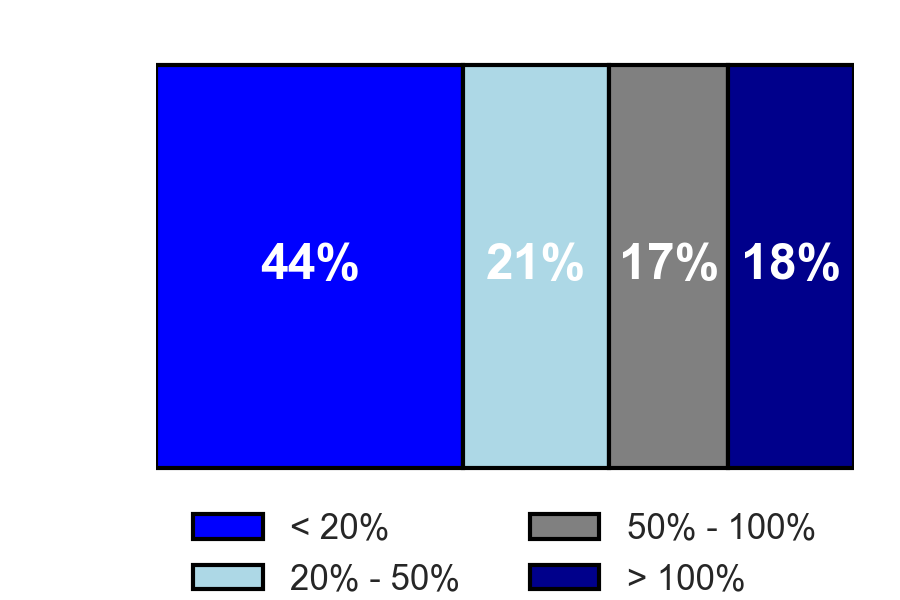
\includegraphics[width=\linewidth]{s3_2021_vol.png}
		\fnote{Source: FTSE-Russell \cite{ftserussell2024}, reporting entities are from the FTSE All-World constituents that disclose S3 emissions}
	\end{subfigure}
\end{figure}

\subsubsection{Lack of consistency and comparability}
In addition to the issues already discussed, there are three reasons why S3 data may not be comparable across firms. First, despite the specifics covered in Section \ref{sec:Scope3Reporting}, the GHG Protocol provides firms with a wide room for manoeuvre regarding which accounting and reporting methodologies they use. For example, firms must make a number of choices including their organisational boundaries, which categories to report, the calculation approach for each category, data sources, how to allocate emissions, whether to report optional extras above the minimum boundaries and so on. As long as these choices can be justified according to the five key accounting principles (which are relevance, completeness, consistency, transparency, accuracy) then they are said to conform to S3 reporting standards \cite{ghgscope32013}. This methodological latitude opens the possibility for meaningful heterogeneity in firms' S3 accounting and reporting: accordingly, while firms may be consistent with respect to themselves, aggregating them into a portfolio risks comparing apples and oranges. 
\\ \\
Second, the GHG Protocol and S3 Guidance is often complimented with standard setters' frameworks and legal rules. While these may intend to be aligned to the GHG Protocol, they invariably introduce particular interpretations and requirements which their signatories are expected to adopt. This could lead to inconsistencies, especially between sectors as they may follow their own industry-specific practices. For example, many financial institutions have adopted the recommendations of the Partnership for Carbon Accounting Financials (PCAF) in an attempt to improve the reporting quality for Category 15 of S3 emissions \cite{PCAF2022}. However, as pointed out by Tang et al. \cite{Tang2023}, the practical considerations of GHG estimation means that PCAF's framework does not align with the reality of availability, reliability and confidence of the ``highest quality'' corporate reported emissions data. This leads to increased non-standardisation, more inaccuracy and further concerns of inconsistency. 
\\ \\
Third, when investors wish to compare the GHG emissions of many firms, perhaps to evaluate the transition risk of their portfolio, they frequently turn to data providers such as Bloomberg, CDP, ISS, MSCI, Sustainalytics, Thomson Reuters, and Trucost. However, due to the previously described problem of missing data, these providers often use estimates to fill in the gaps, but unfortunately each use their own methodologies of varying transparency. These different approaches can compound the inconsistency across the data and make it challenging for people to know what the ``real'' S3 emissions are for a collection of firms. For example, Busch et al. \cite{Busch2022} and Kalesnik et al. \cite{KalesnikVitali2022}  found that third-party estimated data was less consistent than data stemming directly from corporate reports, and so the choice of data provider may significantly affect empirical results. Concerningly, Busch et al. also found that this third-party estimated data inconsistency was increasing over time.  However, this isn't just an issue of estimation methodologies. Even for values reported by firms, surprisingly Nguyen et al. \cite{Nguyenetal2023} found that divergence still exists between third-party datasets, having only 68\% identical data points between Bloomberg and Refinitiv Eikon. 

\section{Estimating S3 emissions}\label{sec:Scope3Modelling}

This Section reviews others' attempts for estimating S3 emissions. Unfortunately, there are not many quantitative papers on S3 emissions in a macro context, such as for a country or industry, due to limited data quality and availability \cite{Hettler2024}. While there are more papers which estimate S1 and S2 emissions, applying these models (for example by transfer learning) is unlikely to yield good results because there is empirically very little relationship between a firm's S1 and S2 emissions versus its reported S3 \cite{ManGroup2022}.   
\\ \\
As there is no industry consensus on the best approach for estimating GHG emissions \cite{FTSERussell2022}, the literature offers several approaches, which Nguyen et al. \cite{nguyen2021} categorise as naive, empirical and ML. We employ this same framework to explore estimation in our S3 context. 

\subsection{Naive estimation}
First, there are naive approaches which all lean heavily on averages. They typically involve several sub-models which are then aggregated or prioritised based on data availability. Common strategies include extrapolation from past emissions, using consumption or production figures, and simple sector averages. While more sophisticated models may be employed for S1 and S2, naive approaches are typically used for S3 estimation by data providers because they are easy to calculate and simple to explain. Companies using such approaches include the ISS \cite{iss2023} and the London Stock Exchange Group (LSEG) \cite{lseg2023}.

\subsection{Empirical estimation}

Empirical estimation encompasses a range of econometric/regression methods which model the linear relationships between variables. While this is a fairly common approach in the literature for estimating S1 and S2 emissions, researchers typically refuse to extend this approach to S3 due to data quality concerns \cite{GoldhammerEtAl2017, KalesnikVitali2022}. 
\\ \\
Nevertheless, a few attempts have been made in a S3 context. For example, the CDP model employs a gamma generalised linear model using revenue and activity information \cite{cdp2023b}. The gamma distribution is chosen due to the positive but heteroskedastic nature of the data. The regressors are the average activity-group revenue intensities reported to the CDP, with revenue broken down into 44 variables. To prevent overfitting, model selection is be optimised by pruning based on activity groupings which chosen to maximise the Akaike Information Criterion (AIC) for each of the 15 S3 categories. Given the hundreds of possible variables that may act as regressors, other variants of linear regression using regularisation are used to automate model selection \cite{CaiXia2023}.
\\ \\
A key drawback for these more traditional statistical approaches is that the estimates rely on parametric assumptions that, if not met, will fail to provide the best, linear, and unbiased estimators. Especially important in the context of Scope 3, \cite{olesiewicz2021} show that if the data is not missing at random then the regression estimates will be biased.

\subsection{Machine learning techniques}

The most common ML approaches are tree-based, often chosen because they combine good performance with model parsimony. In addition, they can handle many of the issues that arise in S3 data, such as missing values and categorical variables. Bloomberg \cite{bloomberg2022} uses a model that estimates S1 and S2 emissions for all industries, and S3 for the oil \& gas and mining sector; it outputs a unique distribution based on comparable companies. They report superior results against both naive and linear models using $R^{2}$ and RMSE measures, but performance halves for firms with average or poor disclosure. 


%%%%%%%%%%%%%%%%%%%%%%%%%%%%%%%%%%%%
\chapter{Project Plan}

Other models to be considered include:
- An autoregressive model (e.g. ARIMA) to see how persistent S3 emissions are. S1 and S2 emissions are highly persistent \cite{KalesnikVitali2022}.
- Simple fixed effects regression using business metrics (as per \cite{KalesnikVitali2022}).

%% bibliography
\bibliographystyle{plain}
\bibliography{references}

\end{document}
